\setlength{\parskip}{\baselineskip}
\section{Theoretical Background}

\begin{frame}
	\huge Theoretical Background
\end{frame}

\begin{frame}{Artificial Neuron}
	\begin{minipage}{0.3\textwidth}
        \begin{figure}[H]
            \centering
    		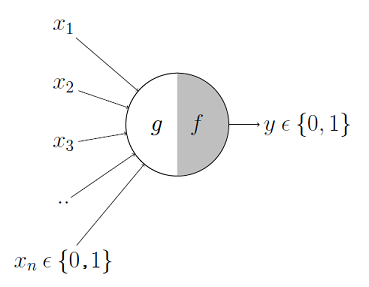
\includegraphics[width=1\textwidth]{Images/Diagrams/McCulloch-Pitts Neuron.png}\\
    		\caption{McCulloch-Pitts Neuron}
    	 \end{figure}
	\end{minipage}%
	\begin{minipage}{0.7\textwidth}
        Fundamental element of Artificial Neural Networks (ANNs)
        \begin{equation*}
        	y = \Phi( b + \sum_{i=1}^{I}x_i*w_i )
        \end{equation*}\\
        
    	\begin{minipage}{0.5\textwidth}
            \centering
            ReLU:
            \begin{equation*}
                \Phi\left( x \right) = \left\{
                	\begin{array}{ll}
                	    0 & x \leq 0\\
                	    x & x > 0\\
                	\end{array} \right.
            \end{equation*}
    	\end{minipage}%
    	\begin{minipage}{0.5\textwidth}
            \centering
            Softmax:
            \begin{equation*}
                \Phi\left( x \right)_{i} = \frac{e^{x_i}}{\sum_{k=1}^{K}e^{x_{j}}}
            \end{equation*}
    	\end{minipage}%
	\end{minipage}%
\end{frame}

\begin{frame}{Deep Neural Network}
    \begin{figure}[H]
        \centering
		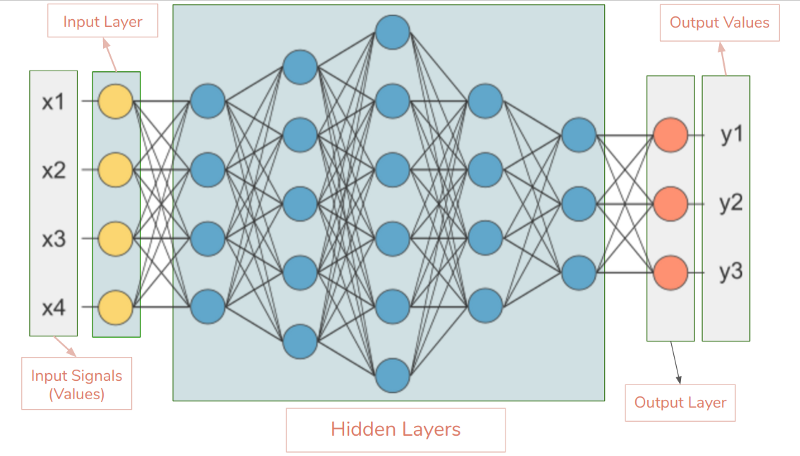
\includegraphics[height=0.8\textheight]{Images/Diagrams/dnn.png}
	 \end{figure}
\end{frame}

\begin{frame}{Convolutional Neural Network}
    \begin{figure}
        \centering
        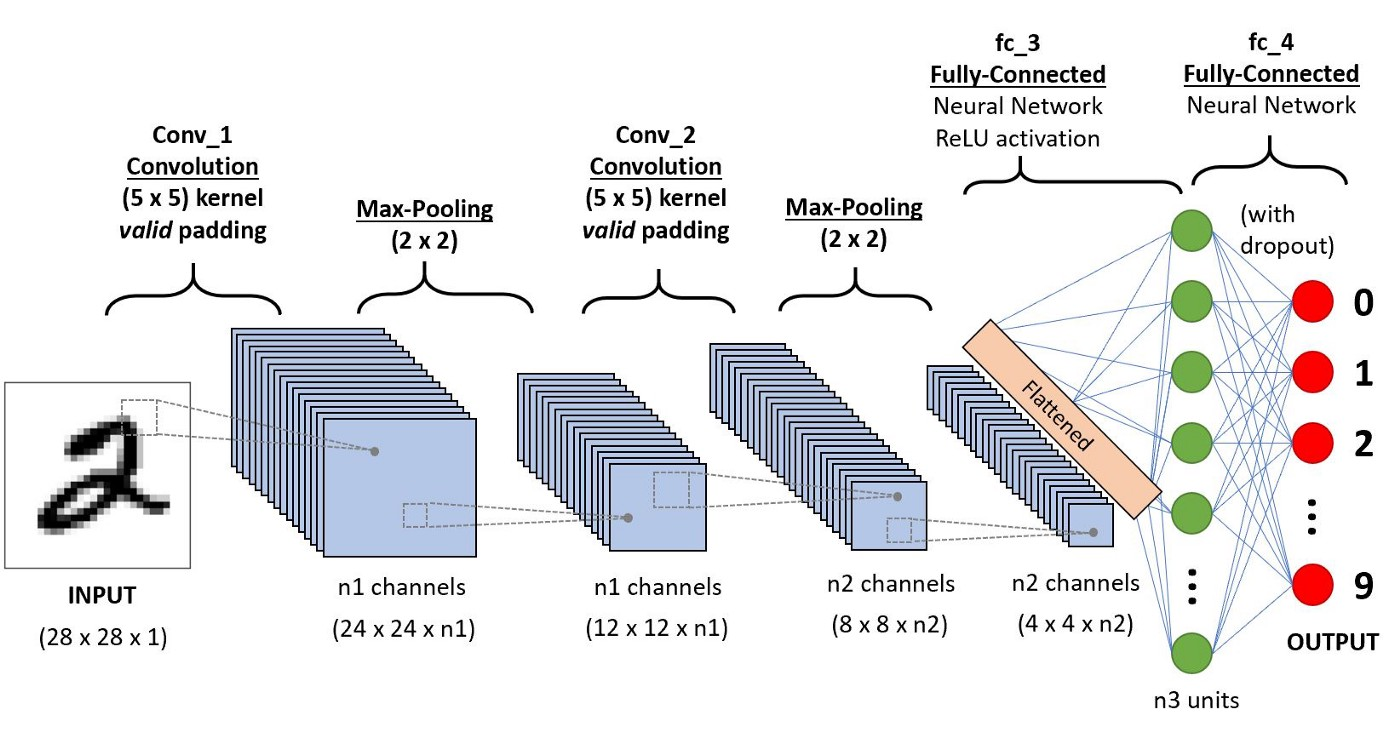
\includegraphics[height=0.85\textheight]{Images/Diagrams/cnn_2conv_layers.jpg}
        \caption{2D convolution}
    \end{figure}
\end{frame}

\begin{frame}{Training Artificial Neural Networks}
    Supervised learning:\\% input-outpout pairs provided
    \begin{enumerate}
        \item forward propagation % ANN makes prediction and calculates error from reality 
        \item back propagation % revert the flow of calculations, to get error per inputs of each layer
        \item calculate gradients % get error per parameters of each layer
        \item update parameters % depending on gradients
    \end{enumerate}
    Batching: Repeats steps 1 to 3 multiple times before running step 4.
\end{frame}

% \begin{frame}{Gradient Descent}
% 	\begin{minipage}{0.5\textwidth}
%         \begin{figure}
%             \centering
%             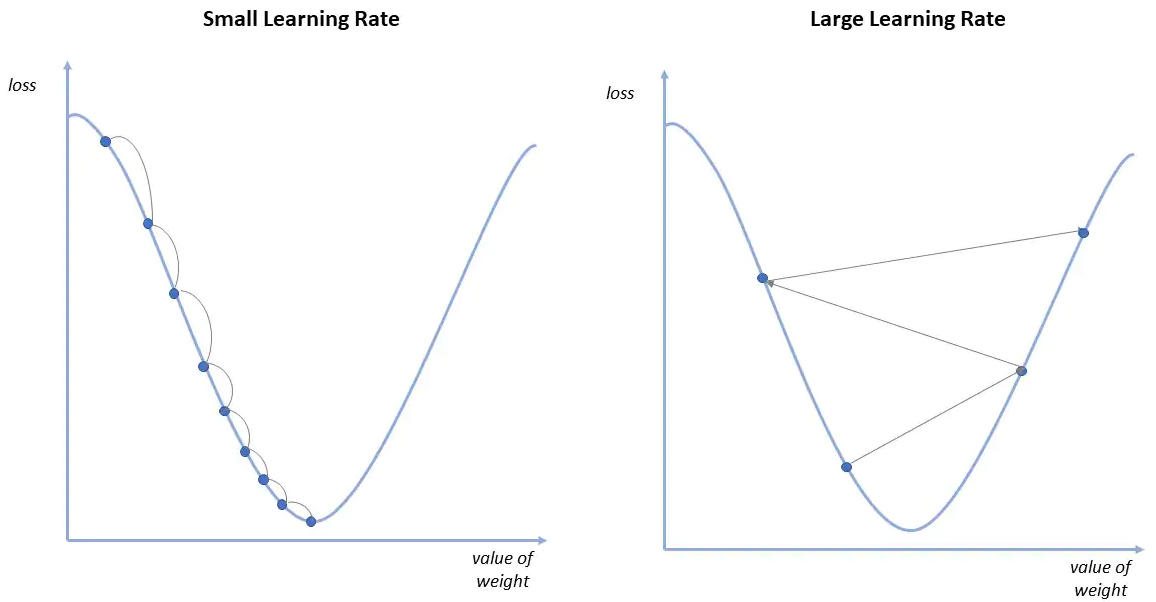
\includegraphics[height=0.5\textheight]{Images/Diagrams/learning_rate.png}
%             \caption{Effect of different learning rates}
%         \end{figure}
% 	\end{minipage}%
% 	\begin{minipage}{0.5\textwidth}
% 	    \centering
%         Gradient Descent with momentum
% 	    \begin{equation*}
%             \begin{gathered} 
%                 m_{n+1} = \beta m_n - \gamma \nabla F \left( a_n + \beta m_n \right)\\
%                 a_{n+1} = a_n + m_{n+1}\\
%             \end{gathered}
%         \end{equation*}
% 	\end{minipage}%
% \end{frame}

% \begin{frame}{Model Overfitting}
%         \begin{figure}
%             \centering
%             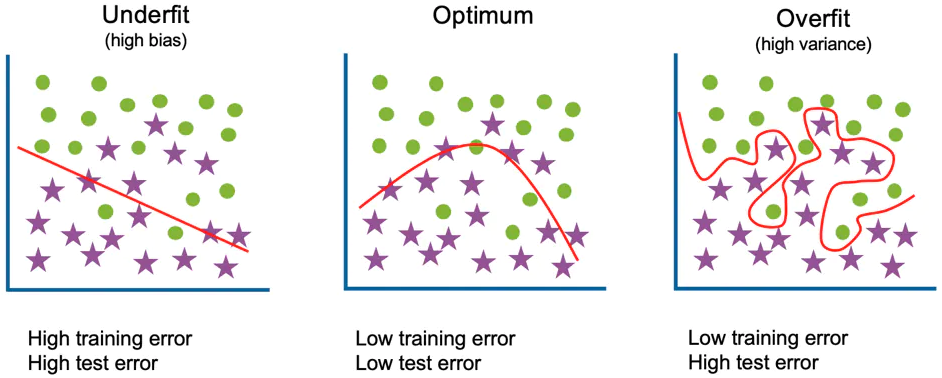
\includegraphics[height=0.6\textheight]{Images/Diagrams/model-over-fitting.png}
%             \caption{Model underfitting and overfitting}
%         \end{figure}
% \end{frame}

\begin{frame}{FL Entities}
	\begin{minipage}{0.5\textwidth}
    	Server:
    	\begin{itemize}
    	    \item model owner
    	    \item orchestrates training
    	    \item no access to any data
    	\end{itemize}
	\end{minipage}%
	\begin{minipage}{0.5\textwidth}
    	Clients:
    	\begin{itemize}
    	    \item data owners
    	    \item train the model
    	    \item share the locally trained model
    	\end{itemize}
	\end{minipage}%
\end{frame}

\begin{frame}{Typical Federated Training Process}
	\begin{minipage}{0.4\textwidth}
        \begin{figure}[H]
            \centering
    		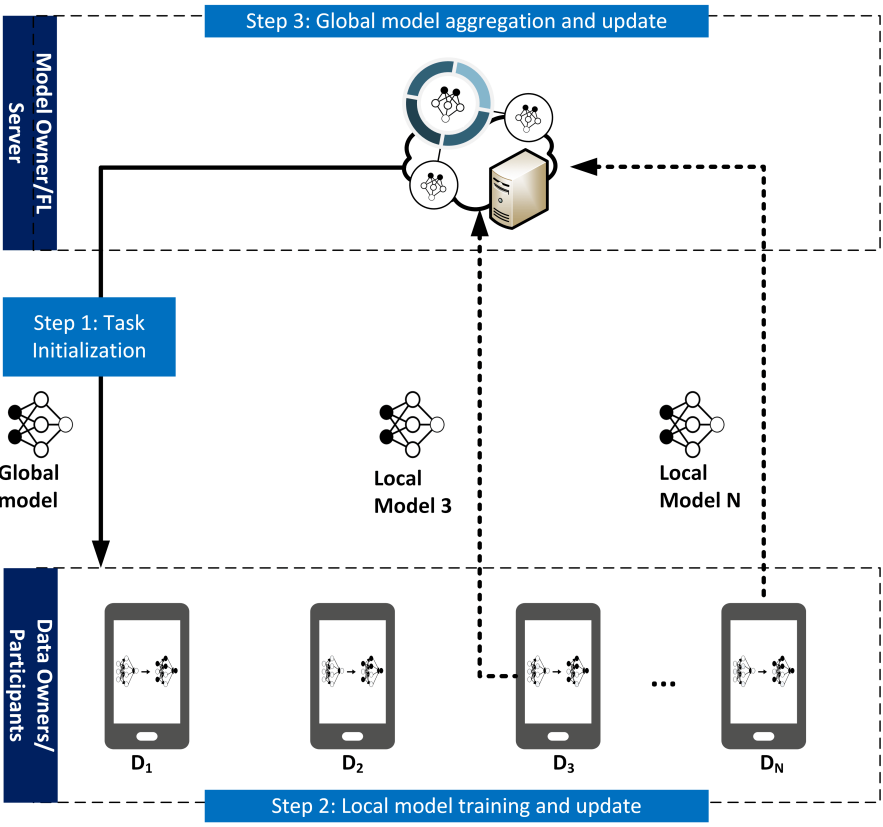
\includegraphics[width=1\textwidth]{Images/Diagrams/fl_topology.png}\\
    		\caption*{Typical FL topology}
		\end{figure}
	\end{minipage}%
	\begin{minipage}{0.6\textwidth}
		\hspace{0.75cm}\textbf{Global Epoch (GE):}
		\begin{enumerate}
		    \item Server broadcast global model to clients.
		    \item Clients generate local models using the global model and their private data.
		    \item Server receives local models and generate new global model.
		\end{enumerate}
	\end{minipage}%
\end{frame}

